% Scientific Book Starter — adapted from minireference/sample-book (MIT),
% a starter template for scientific books with a print-production
% pipeline (Softcover/PolyTeXnic).
%
% SIMPLIFIED SIGNIFICANTLY from upstream: upstream's actual compile path
% requires a Ruby gem (`softcover`, `polytexnic`) to pre-process the .tex
% source before LaTeX ever sees it (the README's own install
% instructions are `gem install` steps, not `pdflatex`), and its 221-line
% softcover.sty plus five auxiliary .sty files load `fontspec` (needing
% xelatex/lualatex) alongside Type1 `helvet`/`courier` fonts (a pdflatex
% assumption) — an internally inconsistent engine requirement that only
% works because the Ruby preprocessor rewrites the source first. This
% starter keeps the STRUCTURE (concept-map-style intro, a mathematics
% fundamentals chapter, front/back matter with an answers section) but
% is a plain, self-contained `book`-class document with ordinary LaTeX
% packages, and entirely original text (the real repo's own chapter
% content is Minireference Co.'s actual published book prose).
\documentclass[10pt]{book}

\usepackage[T1]{fontenc}
\usepackage[svgnames]{xcolor}
\usepackage{graphicx}
\usepackage{amsmath,amssymb,amsthm}
\usepackage{tikz}
\usetikzlibrary{positioning}
\usepackage[colorlinks,linkcolor=DarkBlue,urlcolor=DarkBlue]{hyperref}

\newtheorem{definition}{Definition}[section]
\newtheorem{example}{Example}[section]

\begin{document}

\begin{titlepage}
\centering
\vspace*{3cm}
{\Huge\bfseries Ideas Worth Knowing\par}
\vspace{0.5cm}
{\Large A Short Course in Scientific Thinking\par}
\vspace{2cm}
{\large Priya Anand\par}
\vfill
{\large 2026\par}
\end{titlepage}

\frontmatter
\tableofcontents

%!TEX root = ../main.tex
\chapter*{How This Book Is Organized}
\addcontentsline{toc}{chapter}{How This Book Is Organized}

This book has two short chapters. The first covers the habits of
thought that make scientific reasoning different from ordinary
arguing: making a claim precise enough to be wrong, and checking it
against evidence. The second is a single worked skill, order-of-magnitude
estimation, chosen because it is the fastest way to see those habits
in action.

\begin{center}
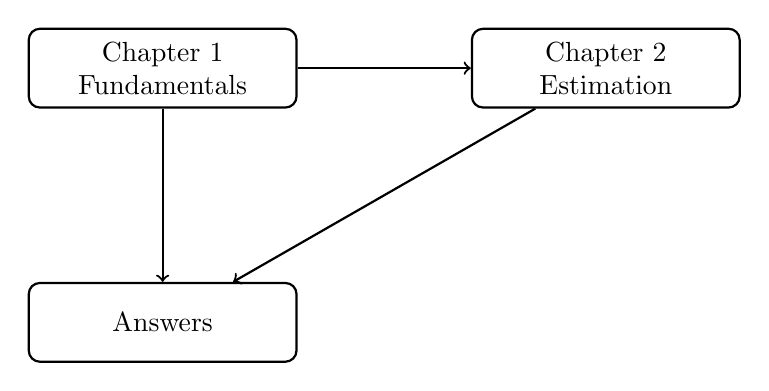
\begin{tikzpicture}[
  node distance=2.2cm,
  box/.style={draw, rounded corners, align=center, minimum width=3.4cm, minimum height=1cm},
  ->, thick
]
\node[box] (fund) {Chapter 1\\Fundamentals};
\node[box, right=of fund] (est) {Chapter 2\\Estimation};
\node[box, below=of fund] (ans) {Answers};
\draw (fund) -- (est);
\draw (fund) -- (ans);
\draw (est) -- (ans);
\end{tikzpicture}
\end{center}

%!TEX root = ../main.tex
\chapter*{Preface}
\addcontentsline{toc}{chapter}{Preface}

This book grew out of a two-lecture unit I taught to students who were
not planning to become scientists but wanted to know how scientists
decide what to believe. It assumes no mathematics beyond arithmetic
and a willingness to be wrong out loud, which turns out to be the
harder of the two requirements.


\mainmatter

%!TEX root = ../main.tex
\chapter{Fundamentals}
\label{ch:fundamentals}

Scientific thinking is not a personality trait; it is a small set of
habits that anyone can practice. This chapter covers two of them:
making a claim precise, and checking it against evidence.

\section{Making a Claim Precise}
\label{sec:precise-claims}

\begin{definition}[Falsifiable claim]
A claim is \emph{falsifiable} if there exists some observation that,
were it made, would show the claim to be false.
\end{definition}

``This medicine helps some people'' is not falsifiable in any useful
sense — almost any outcome is compatible with it. ``This medicine
reduces average recovery time by at least two days, in a controlled
trial with a placebo arm'' is falsifiable: a trial could come back
showing no difference, or a difference smaller than two days.

\begin{example}
Compare ``vitamin C prevents colds'' with ``taking 1000mg of vitamin C
daily reduces the annual number of colds in adults by more than 20\%,
measured against a placebo control.'' The second version can actually
be tested — and, when it has been, the reduction found is usually much
smaller than folklore suggests.
\end{example}

\section{Checking Against Evidence}
\label{sec:evidence}

Precision alone is not enough; the claim also has to be checked
against an observation that could, in principle, have gone the other
way. A prediction confirmed only by evidence you already knew about
before making the prediction does not count — this is sometimes called
\emph{postdiction} rather than prediction, and it is far easier to get
right by accident.

%!TEX root = ../main.tex
\chapter{Order-of-Magnitude Estimation}
\label{ch:estimation}

Physicist Enrico Fermi was famous for estimating quantities he had no
direct data for — the number of piano tuners in Chicago, say — by
breaking the question into smaller pieces that could each be guessed
within a factor of two or three, and multiplying them together. The
errors in the pieces tend to partially cancel, and the final estimate
usually lands within an order of magnitude of the truth.

\section{A Worked Example}
\label{sec:worked-example}

\begin{example}[How many leaves are on a large oak tree?]
Estimate: a mature oak canopy is roughly a sphere 15 metres across.
A branch tip carries perhaps 20 leaves in a cluster the size of a
fist, and clusters are spaced roughly 10cm apart across the outer
surface of the canopy. The canopy's surface area is about
$4\pi (7.5\,\text{m})^2 \approx 700\,\text{m}^2$. At one cluster per
$0.01\,\text{m}^2$ of surface, that's about 70{,}000 clusters, and
$70{,}000 \times 20 \approx 1.4$ million leaves — comfortably in the
range (100{,}000 to a few million) that direct counts of oak trees
actually report.
\end{example}

\section{Why the Errors Cancel}
\label{sec:why-errors-cancel}

Each individual guess in the chain above could easily be off by a
factor of two. But an overestimate in one factor is roughly as likely
as an underestimate, and independent errors of that size tend not to
all point the same direction at once. This is why a chain of five
rough guesses, each uncertain by a factor of two, typically lands the
final answer within a factor of three or four of the truth — far
better than the naive intuition that the errors should simply
multiply together.


\backmatter

%!TEX root = ../main.tex
\chapter{Answers and Notes}
\label{ch:answers}

\textbf{Chapter~\ref{ch:fundamentals}, Section~\ref{sec:precise-claims}.}
The vitamin C example is drawn from the Cochrane systematic reviews on
vitamin C and the common cold, which found a reduction in cold
duration but essentially no reduction in incidence for the general
population.

\textbf{Chapter~\ref{ch:estimation}, Section~\ref{sec:worked-example}.}
Try the same method on a question of your own choosing — how many
words are in your favourite novel, or how many bricks are in a
building you walk past daily — and compare your estimate against a
real count if one is available.


\end{document}
